\documentclass[10pt]{beamer}
\usetheme[
%%% option passed to the outer theme
%    progressstyle=fixedCircCnt,   % fixedCircCnt, movingCircCnt (moving is deault)
  ]{Feather}
  
% If you want to change the colors of the various elements in the theme, edit and uncomment the following lines

% Change the bar colors:
%\setbeamercolor{Feather}{fg=red!20,bg=red}

% Change the color of the structural elements:
%\setbeamercolor{structure}{fg=red}

% Change the frame title text color:
%\setbeamercolor{frametitle}{fg=blue}

% Change the normal text color background:
%\setbeamercolor{normal text}{fg=black,bg=gray!10}

%-------------------------------------------------------
% INCLUDE PACKAGES
%-------------------------------------------------------

\usepackage[utf8]{inputenc}
\usepackage[english]{babel}
\usepackage[T1]{fontenc}
\usepackage{helvet}
\usepackage[document]{ragged2e}
\usepackage{graphicx}
\usepackage[rightcaption]{sidecap}
\usepackage[none]{hyphenat}
\usepackage{animate,media9,movie15}

%-------------------------------------------------------
% DEFFINING AND REDEFINING COMMANDS
%-------------------------------------------------------

% colored hyperlinks
\newcommand{\chref}[2]{
  \href{#1}{{\usebeamercolor[bg]{Feather}#2}}
}

%-------------------------------------------------------
% INFORMATION IN THE TITLE PAGE
%-------------------------------------------------------

\title[] % [] is optional - is placed on the bottom of the sidebar on every slide
{ % is placed on the title page
      \textbf{Ventanas Inteligentes}
}

\subtitle[Ventanas Inteligentes]
{
      \textbf{}
}

\author[]
{      Francisco Javier MendozaBautista\\
      {\ttfamily fj.mendozabautista@ugto.mx}
}

\institute[]
{
     Universidad de Guanajuato \\Ingeniería Electrónica\\
  
  %there must be an empty line above this line - otherwise some unwanted space is added between the university and the country (I do not know why;( )
}

\date{\today}

%-------------------------------------------------------
% THE BODY OF THE PRESENTATION
%-------------------------------------------------------

\begin{document}

%-------------------------------------------------------
% THE TITLEPAGE
%-------------------------------------------------------

{\1% % this is the name of the PDF file for the background
\begin{frame}[plain,noframenumbering] % the plain option removes the header from the title page, noframenumbering removes the numbering of this frame only
  \titlepage % call the title page information from above
\end{frame}}


\begin{frame}{Contenido}{}
\tableofcontents
\end{frame}

%-------------------------------------------------------
\section{Ventanas inteligentes}
%-------------------------------------------------------
\subsection{¿Que son las ventanas inteligentes?}
\begin{frame}{Ventanas inteligentes}{¿Que son las ventanas inteligentes?}

\begin{columns}
	\column{0.5\textwidth}
	\justify
	Se trata de unas ventana que tienen incorporado un sistema que en cuestión de segundos, mediante un interruptor, se puede activar una tecnología que provoca unas reacciones químicas y físicas haciendo que el vidrio transparente se convierta en opaco
	\column{0.5\textwidth}
    \begin{figure}
    	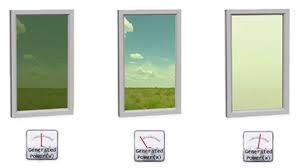
\includegraphics[scale=0.5]{Imagenes/1}
    	\caption{Ventanas inteligentes}
    \end{figure}
\end{columns}
\end{frame}

\subsection{¿Como funcionan?}
\begin{frame}{Ventanas inteligentes}{Externally Modulated Displays}


  \begin{columns}
  	\column{0.5\textwidth}

  	  \begin{figure}
  	  	
\includegraphics[scale=0.5]{Imagenes/2}
  	  	\caption{CSIC}
  	  \end{figure}
  	\column{0.5\textwidth}
      	\justify
    En lugar de utilizar cristal líquido, las ventanas inteligentes desarrolladas por el CSIC aplican una tecnología basada en la activación controlada de una combinación de reacciones químicas y físicas que permiten oscurecer o volver transparentes los cristales.
  \end{columns} 

\end{frame}

\subsection{¿Como funcionan?}
\begin{frame}{Ventanas inteligentes}{¿Como funcionan?}
    \justify	
    Su funcionamiento consiste en películas delgadas de material poroso que al ser expuesto a la humedad o la sequedad del ambiente cambian su transmisión óptica consiguiendo que las ventanas se vuelvan opacas o transparentes. De esta manera, la ventana regula la cantidad de luz que entra a través del cristal.
    Controlando el grado de humedad de la corriente de aire que circula por los cristales, el usuario  puede activar o desactivar a su antojo la transparencia de las ventanas de su hogar, oficina o negocio para ver u ocultar el interior de la estancia. El tiempo de respuesta es de cuestión de unos pocos segundos.

\end{frame}


\subsection{Ventajas}
\begin{frame}{Ventanas inteligentes}{Ventajas}
    
    \begin{columns}
    	\column{0.5\textwidth}
    	\justify 
    	Las ventanas inteligentes  no requieren ninguna adaptación a las normativas vigentes, puesto que se trata únicamente de una variación en el vidrio que se utiliza en la actualidad. Además, provocan un gran ahorro en aire acondicionado durante los meses de calor, ya que al regular la cantidad de luz solar que penetra en la casa o en la oficina se puede reducir la temperatura del ambiente sin necesidad de bajar las persianas y encender la luz.

    	\column{0.5\textwidth}
        \begin{figure}
        	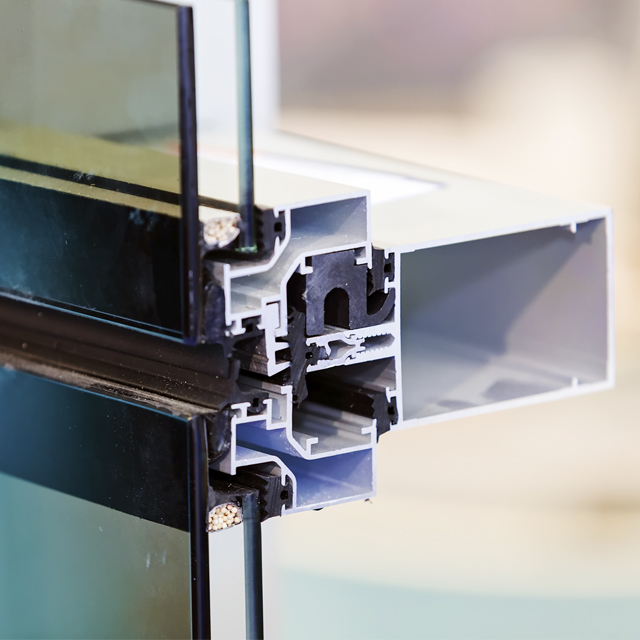
\includegraphics[scale=0.2]{Imagenes/3}
        \caption{Ventana}
        \end{figure}
    \end{columns} 
\end{frame}




\subsection{Video}
\begin{frame}{Ventanas inteligentes}{Video}
   

%   	   \begin{figure}
%   		%    \movie[width=3cm,height=3cm,poster]{}{Wildlife.wmv}
%   		%    \animategraphics[controls,autoplay,loop,scale=0.5]{10}{Wildlife}{}{}
%   		%    \includemovie[autoplay]{Wildlife.wmv}

\begin{figure}		
   		\includemovie[
   		poster,
   		autoplay,
   	    externalviewer,
   		inline=false,
   		text={\small(click)}
   		]{6cm}{6cm}{video.mp4}
   		
   		%    \flashmovie{Wildlife.wmv}
   	\end{figure}
 

\end{frame}


\end{document}